\documentclass{article}
\usepackage{tikz,amsmath}
\title{CSC 320 Assignment 2}
\author{Oliver Tonnesen\\V00885732}
\date{February 17, 2019}
\begin{document}
\maketitle
\renewcommand{\thesubsection}{\thesection.\alph{subsection}}
\section{} % Section 1
Let $w=1^{2p}$, where $p$ is the pumping length of $L$. Let $w=xyz$ where
$x=1^i$, $y=1^j$, and $z=1^k$. To satisfy the conditions of the pumping lemma,
we have $i+j\le p$, and so $k=2p-i-j\ge p$. The pumping lemma then asserts that
$xy^lz\in L\;\forall l\ge0$. So
\[1^i(1^j)^l1^k\in L\;\forall l\ge0.\]
So $|w|=i+jl+k$. Let $l=i+k$. Then
\begin{align*}
	|w|&=i+j(i+k)+k\\
	&=i+ij+jk+k\\
	&=i(1+j)+k(j+1)\\
	&=(i+k)(j+1)
\end{align*}
Recall that $k\ge p$ and also note that $|y|=j>0$, so both $i+k$ and $j+1$ are
larger than 1. Thus, $(i+k)(j+1)$ must be a composite number (in other words,
$1^{(i+k)(j+1)}\not\in L$) and so $L$ is not regular.
\section{} % Section 2
Let $s=1^{2p}$ where $p$ is the pumping length of $L$. Let $s=uvwxy$ where
$u=1^i$, $v=1^j$, $w=1^k$, $x=1^l$, and $y=1^m$. To satisfy the conditions of
the pumping lemma, we have $j+k+l\le p$, and so $i+m=2p-j-k-l\ge p$. The
pumping lemma then asserts that $uv^nwx^ny\in L\;\forall n\ge0$. So
\[1^i(1^j)^n1^k(1^l)^n1^m\in L\;\forall n\ge0.\]
So $|s|=i+jn+k+ln+m$. Let $n=i+k+m$. Then
\begin{align*}
	|s|&=i+k+m+n(j+l)\\
	&=i+k+m+(i+k+m)(j+l)\\
	&=(i+k+m)(j+l+1)
\end{align*}
Recall that $i+m\ge p$ and also note that $|vx|=j+l>0$, so both $i+k+m$ and
$j+l+1$ are larger than 1. Thus, $(i+k+m)(j+l+1)$ must be a composite number
(in other words, $1^{(i+k+m)(j+l+1)}\not\in L$) and so $L$ is not context-free.
\section{} % Section 3
The $CFG$ for $L$:
\begin{align*}
	(\{S\},\{a,b,\varepsilon,\emptyset,(,),\cup,\circ,*\},
	\{S\rightarrow a,S\rightarrow b,S\rightarrow\varepsilon,S\rightarrow\emptyset,\\
	S\rightarrow(S\cup S),S\rightarrow(S\circ S),S\rightarrow(S^*)\},S)
\end{align*}
Here are the language's productions in a more readable format:
\begin{align*}
	S&\rightarrow a\\
	S&\rightarrow b\\
	S&\rightarrow\varepsilon\\
	S&\rightarrow\emptyset\\
	S&\rightarrow(S\cup S)\\
	S&\rightarrow(S\circ S)\\
	S&\rightarrow(S^*)
\end{align*}
\section{} % Section 4
\subsection{} % Section 4.a
$G$ in Chomsky Normal Form:
\begin{align*}
	(\{S_0,S,A,B,S_A,S_B\},\{a,b,\varepsilon\},
	\{S_0\rightarrow\varepsilon,A\rightarrow a,B\rightarrow b,S_0\rightarrow AS_A,\\
	S\rightarrow AS_A,S_A\rightarrow SA,S_0\rightarrow BS_B,S\rightarrow BS_B,\\
	S_B\rightarrow SB,S_0\rightarrow AA,S\rightarrow BB,S_0\rightarrow BB, S\rightarrow AA\},S_0)
\end{align*}
Again, the language's productions in a more readable format:
\begin{align*}
	S_0&\rightarrow\varepsilon\\
	A&\rightarrow a\\
	B&\rightarrow b\\
	S_0&\rightarrow AS_A\\
	S&\rightarrow AS_A\\
	S_A&\rightarrow SA\\
	S_0&\rightarrow BS_B\\
	S&\rightarrow BS_B\\
	S_B&\rightarrow SB\\
	S_0&\rightarrow AA\\
	S&\rightarrow BB\\
	S_0&\rightarrow BB\\
	S&\rightarrow AA\\
\end{align*}
\subsection{} % Section 4.b
\begin{tabular}{|c|c|c|c|c|c|c|}
	\hline
	6 & $\{S_0,S\}$ &  &  &  &  & \\
	\hline
	5 & $\emptyset$ & $\{S_A\}$ &  &  &  & \\
	\hline
	4 & $\emptyset$ & $\{S_0,S\}$ & $\emptyset$ &  &  & \\
	\hline
	3 & $\emptyset$ & $\{S_B\}$ & $\{S_B\}$ & $\{S_A\}$ &  & \\
	\hline
	2 & $\emptyset$ & $\{S_0,S\}$ & $\{S_0,S\}$ & $\{S_0,S\}$ & $\emptyset$ & \\
	\hline
	1 & $\{A\}$ & $\{B\}$ & $\{B\}$ & $\{B\}$ & $\{B\}$ & $\{A\}$ \\
	\hline
	& a & b & b & b & b & a \\
	\hline
\end{tabular}
\newline
\newline
There is a start variable in the top rightmost cell of the table, so $abbbba$
is in the language.
\section{} % Section 5
The general idea is to push two 1s onto the stack for each 1 seen, and to pop
one 1 for each 0 seen. We accept only when there are no 1s left on the stack
when we reach the end of the input.
\newline
\begin{minipage}{\textwidth}
\begin{center}
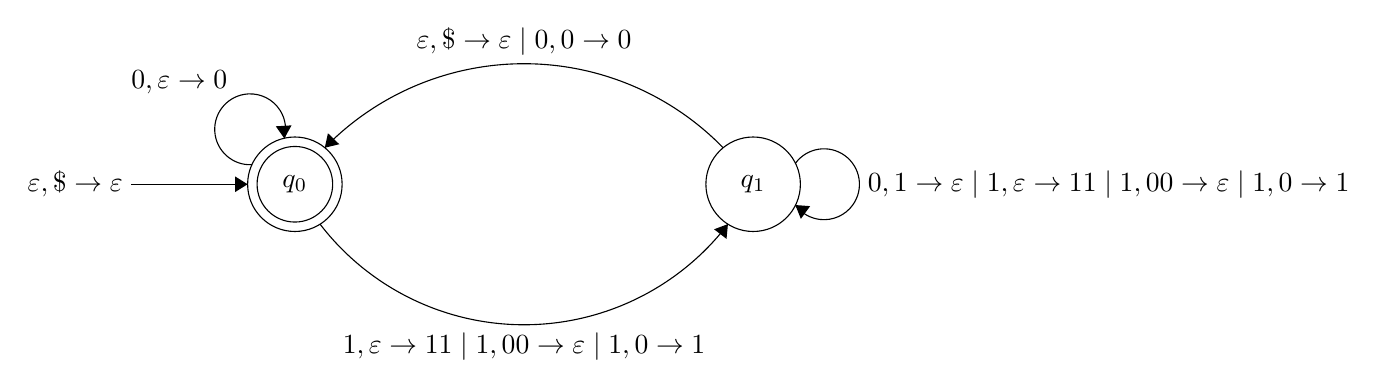
\begin{tikzpicture}[scale=0.2]
\tikzstyle{every node}+=[inner sep=0pt]
\draw [black] (20.6,-24.6) circle (3);
\draw (20.6,-24.6) node {$q_0$};
\draw [black] (20.6,-24.6) circle (2.4);
\draw [black] (49.7,-24.6) circle (3);
\draw (49.7,-24.6) node {$q_1$};
\draw [black] (17.883,-23.357) arc (273.14993:-14.85007:2.25);
\draw (13.26,-18.87) node [above] {$0,\varepsilon\rightarrow0$};
\fill [black] (19.93,-21.69) -- (20.39,-20.86) -- (19.39,-20.92);
\draw [black] (10.2,-24.6) -- (17.6,-24.6);
\draw (9.7,-24.6) node [left] {$\varepsilon,\$\rightarrow\varepsilon$};
\fill [black] (17.6,-24.6) -- (16.8,-24.1) -- (16.8,-25.1);
\draw [black] (22.501,-22.284) arc (135.75774:44.24226:17.657);
\fill [black] (22.5,-22.28) -- (23.42,-22.06) -- (22.7,-21.36);
\draw (35.15,-16.45) node [above] {$\varepsilon,\$\rightarrow\varepsilon\;|\;0,0\rightarrow0$};
\draw [black] (48.103,-27.134) arc (-37.49012:-142.50988:16.324);
\fill [black] (48.1,-27.13) -- (47.22,-27.46) -- (48.01,-28.07);
\draw (35.15,-34.02) node [below] {$1,\varepsilon\rightarrow11\;|\;1,00\rightarrow\varepsilon\;|\;1,0\rightarrow1$};
\draw [black] (52.38,-23.277) arc (144:-144:2.25);
\draw (56.95,-24.6) node [right] {$0,1\rightarrow\varepsilon\;|\;1,\varepsilon\rightarrow11\;|\;1,00\rightarrow\varepsilon\;|\;1,0\rightarrow1$};
\fill [black] (52.38,-25.92) -- (52.73,-26.8) -- (53.32,-25.99);
\end{tikzpicture}
\end{center}

\end{minipage}
\section{} % Section 6
We read the first copy of $w$ onto the first stack. At some point, we ``guess''
that we're in the middle of the string when we read a 1. We now pop all of $w$
off of the first stack and onto the second stack. We now have a copy of $w$
``backwards'' (as in the last letter is on the bottom, and the first letter is
on the top) on the second stack. We compare each of these to what remains of
the string, and accept when we find the bottom of the second stack with no
input left.
\newline
\newline
Here our transitions work as follows:
\[(\lambda,a,b)\rightarrow(\alpha,\beta)\]
reads $\lambda$ from the input, pops $a$ from stack 1 and pops $b$ from stack 2,
then pushes $\alpha$ onto stack 1 and pushes $\beta$ onto stack 2.
\newline
\newline
\begin{minipage}{\textwidth}
\begin{center}
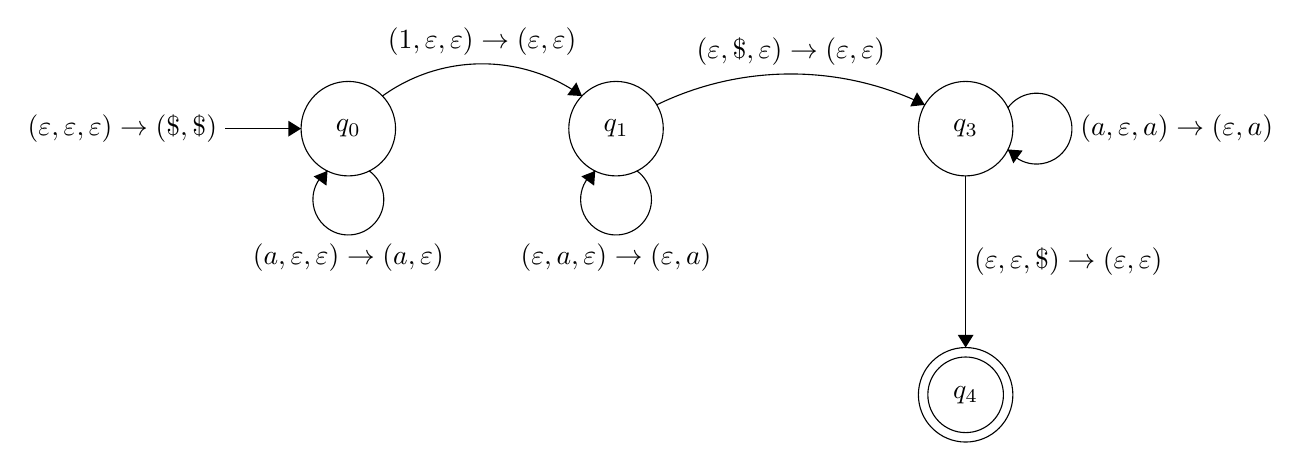
\begin{tikzpicture}[scale=0.2]
\tikzstyle{every node}+=[inner sep=0pt]
\draw [black] (20.5,-27.3) circle (3);
\draw (20.5,-27.3) node {$q_0$};
\draw [black] (37.5,-27.3) circle (3);
\draw (37.5,-27.3) node {$q_1$};
\draw [black] (59.7,-27.3) circle (3);
\draw (59.7,-27.3) node {$q_3$};
\draw [black] (59.7,-44.2) circle (3);
\draw (59.7,-44.2) node {$q_4$};
\draw [black] (59.7,-44.2) circle (2.4);
\draw [black] (21.823,-29.98) arc (54:-234:2.25);
\draw (20.5,-34.55) node [below] {$(a,\varepsilon,\varepsilon)\rightarrow(a,\varepsilon)$};
\fill [black] (19.18,-29.98) -- (18.3,-30.33) -- (19.11,-30.92);
\draw [black] (12.7,-27.3) -- (17.5,-27.3);
\draw (12.2,-27.3) node [left] {$(\varepsilon,\varepsilon,\varepsilon)\rightarrow(\$,\$)$};
\fill [black] (17.5,-27.3) -- (16.7,-26.8) -- (16.7,-27.8);
\draw [black] (22.66,-25.232) arc (125.83003:54.16997:10.831);
\fill [black] (35.34,-25.23) -- (34.98,-24.36) -- (34.4,-25.17);
\draw (29,-22.68) node [above] {$(1,\varepsilon,\varepsilon)\rightarrow(\varepsilon,\varepsilon)$};
\draw [black] (38.823,-29.98) arc (54:-234:2.25);
\draw (37.5,-34.55) node [below] {$(\varepsilon,a,\varepsilon)\rightarrow(\varepsilon,a)$};
\fill [black] (36.18,-29.98) -- (35.3,-30.33) -- (36.11,-30.92);
\draw [black] (40.087,-25.786) arc (115.92542:64.07458:19.473);
\fill [black] (57.11,-25.79) -- (56.61,-24.99) -- (56.18,-25.89);
\draw (48.6,-23.33) node [above] {$(\varepsilon,\$,\varepsilon)\rightarrow(\varepsilon,\varepsilon)$};
\draw [black] (62.38,-25.977) arc (144:-144:2.25);
\draw (66.95,-27.3) node [right] {$(a,\varepsilon,a)\rightarrow(\varepsilon,a)$};
\fill [black] (62.38,-28.62) -- (62.73,-29.5) -- (63.32,-28.69);
\draw [black] (59.7,-30.3) -- (59.7,-41.2);
\fill [black] (59.7,-41.2) -- (60.2,-40.4) -- (59.2,-40.4);
\draw (60.2,-35.75) node [right] {$(\varepsilon,\varepsilon,\$)\rightarrow(\varepsilon,\varepsilon)$};
\end{tikzpicture}
\end{center}

\end{minipage}
\section{} % Section 7
\subsection{} % Section 7.a
\begin{minipage}{\textwidth}
\begin{center}
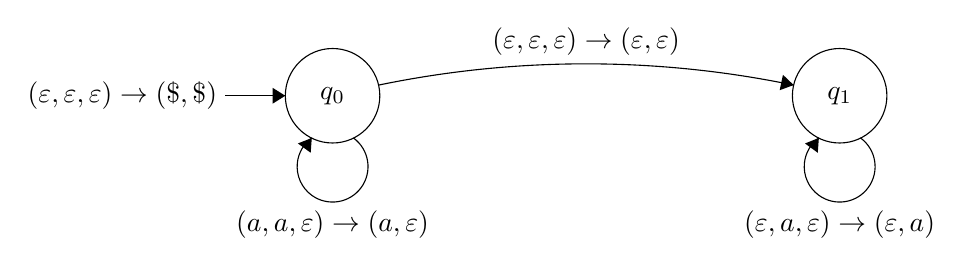
\begin{tikzpicture}[scale=0.2]
\tikzstyle{every node}+=[inner sep=0pt]
\draw [black] (24.1,-25.7) circle (3);
\draw (24.1,-25.7) node {$q_0$};
\draw [black] (56.3,-25.7) circle (3);
\draw (56.3,-25.7) node {$q_1$};
\draw [black] (17.3,-25.7) -- (21.1,-25.7);
\draw (16.8,-25.7) node [left] {$(\varepsilon,\varepsilon,\varepsilon)\rightarrow(\$,\$)$};
\fill [black] (21.1,-25.7) -- (20.3,-25.2) -- (20.3,-26.2);
\draw [black] (25.423,-28.38) arc (54:-234:2.25);
\draw (24.1,-32.95) node [below] {$(a,a,\varepsilon)\rightarrow(a,\varepsilon)$};
\fill [black] (22.78,-28.38) -- (21.9,-28.73) -- (22.71,-29.32);
\draw [black] (27.022,-25.024) arc (101.7088:78.2912:64.934);
\fill [black] (53.38,-25.02) -- (52.7,-24.37) -- (52.49,-25.35);
\draw (40.2,-23.17) node [above] {$(\varepsilon,\varepsilon,\varepsilon)\rightarrow(\varepsilon,\varepsilon)$};
\draw [black] (57.623,-28.38) arc (54:-234:2.25);
\draw (56.3,-32.95) node [below] {$(\varepsilon,a,\varepsilon)\rightarrow(\varepsilon,a)$};
\fill [black] (54.98,-28.38) -- (54.1,-28.73) -- (54.91,-29.32);
\end{tikzpicture}
\end{center}

\end{minipage}
\subsection{} % Section 7.b
The double pushdown automaton would use the following transition:
\[(q,A,\varepsilon,A)\rightarrow\{(p,B,\varepsilon\}\]
First, we move from state $q$ to $p$. Then (more importantly) we pop $A$ from
stack 2 (the portion of the ``tape'' to the right of the ``tape head'') and
push $B$ onto stack 1, simulating writing to the tape and moving one cell
to the right.
\end{document}
